
%***************************************************************************
%
% CreditCruncher - A portfolio credit risk valorator
% Copyright (C) 2004 Gerard Torrent
%
% This program is free software; you can redistribute it and/or
% modify it under the terms of the GNU General Public License
% as published by the Free Software Foundation; either version 2
% of the License.
%
% This program is distributed in the hope that it will be useful,
% but WITHOUT ANY WARRANTY; without even the implied warranty of
% MERCHANTABILITY or FITNESS FOR A PARTICULAR PURPOSE.  See the
% GNU General Public License for more details.
%
% You should have received a copy of the GNU General Public License
% along with this program; if not, write to the Free Software
% Foundation, Inc., 59 Temple Place - Suite 330, Boston, MA 02111-1307, USA.
%
%
% introduction.tex - TeX documentation file
% --------------------------------------------------------------------------
%
% 2004/12/04 - Gerard Torrent [gerard@fobos.generacio.com]
%   . initial release
%
%***************************************************************************

\chapter{Introducci\'on}
\label{sec:introduction}

\section{About CreditCruncher}

CreditCruncher valora el riesgo de impago de una cartera de cr\'editos usando la 
t\'ecnica de simulaci\'on Monte Carlo. Es una implementaci\'on libre de la metodologia
CreditMetrics\footnote{http://www.riskmetrics.com/}. 

Se dispone de una cartera de N clientes donde cada cliente tiene contratado uno o 
varios productos con riesgo de cr\'edito. Cada cliente tiene asignado un rating de 
calidad crediticia y existe una matriz de transici\'on que permite determinar la 
probabilidad de fallido a un horizonte de tiempo fijado. Los clientes pertenecen 
a diversos sectores de los que disponemos de una matriz de correlaci\'on que 
indica el grado de dependencia intersectorial en caso de fallido. A partir de 
la matriz de correlaci\'on intersectorial se construye la matriz de correlaci\'on 
entre clientes. Finalmente se genera un conjunto de N variables aleatorias 
uniformes correlacionadas seg\'un esta matriz (c\'opula). Se usa la matriz de 
transici\'on para determinar la evoluci\'on del rating inicial de cada cliente y se 
evalua el valor de sus productos. Si se repite este proceso un n\'umero elevado de 
veces disponemos de un conjunto de valores posibles de la cartera que permiten 
determinar la distribuci\'on del valor de la cartera y calcular el VAR (Value At Risk). 
Para mas informaci\'on cons\'ultese el manual de CreditCruncher donde se describe 
con detalle todos los pasos realizados.\cite{Ait-83,Cum-97}

\begin{figure}[!hb]
\begin{center}

\includegraphics[height=5cm, angle=0]{./images/copula.eps}
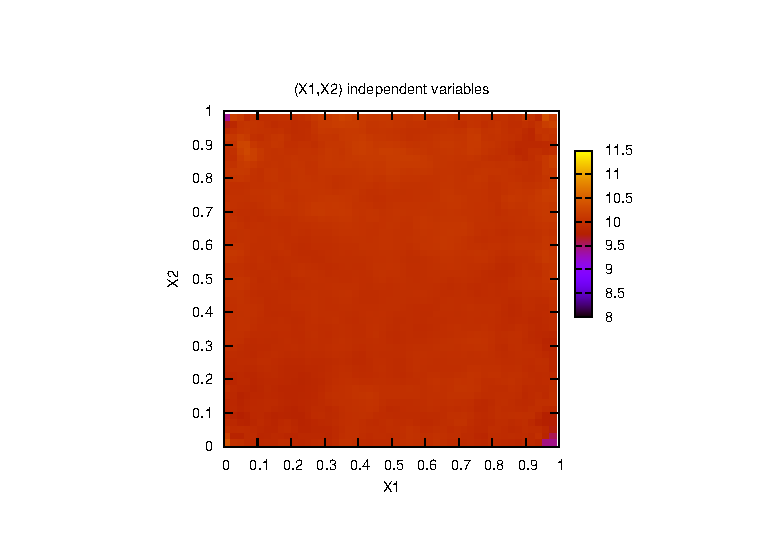
\includegraphics[height=5cm, angle=0]{./images/uniform.eps}
\caption{Bivariate distribution plot with correlation and independent}
\label{fig1}
\end{center}
\end{figure}

\section{Modelos de valoraci\'on del riesgo de cr\'edito}

Se recomienda la lectura del excelente art\'iculo \emph{Different strokes}
\cite{Risk:Dif_Str} donde se exponen los modelos de valoraci\'on del 
risgo de cr\'edito y sus principales caracter\'isticas. 


